\section{Total Variance Minimization (TVM)}

TVM, bir görüntünün pikselleri arasındaki ani değişiklikleri (keskin kenarları) en aza indirmeye çalışır. TVM, görüntüdeki pikseller arasındaki varyasyonu azaltarak, adversarial örneklerin görüntü üzerindeki etkilerini minimuma indirmeyi hedefler. 

TVM, bir görüntünün toplam varyansını minimize ederek çalışır. Bu işlem sırasında, komşu pikseller arasındaki farkların toplamı minimize edilmeye çalışılır. Bu farklar "total variation" adı verilen bir fonksiyon ile ölçülür. Total variation, görüntüdeki komşu pikseller arasındaki farkların toplamı olarak adlandırılır. Görüntüdeki pikseller arasındaki keskin geçişler ve değişiklikler bu işlemle azaltılır. TVM, bir görüntüyü iki bileşene ayırır:

\begin{itemize}
    \item \textbf{Yüksek Frekanslı Bileşenler}: Gürültü ve adversarial saldırılar tarafından eklenen küçük değişiklikler.
    \item \textbf{Düşük Frekanslı Bileşenler}: Orijinal görüntü bilgisi.
\end{itemize}

Amaç, yüksek frekanslı gürültüleri azaltarak görüntünün düşük frekanslı bileşenlerine odaklanmaktır.

\subsubsection{Python Kodu}

\begin{lstlisting}[language=Python]
from art.defences.preprocessor import TotalVarMin

tv_minimization = TotalVarMin(clip_values=(min_, max_))
def_test, _ = tv_minimization(adv_test, y_test)
\end{lstlisting}

\begin{figure}[h]
    \centering
    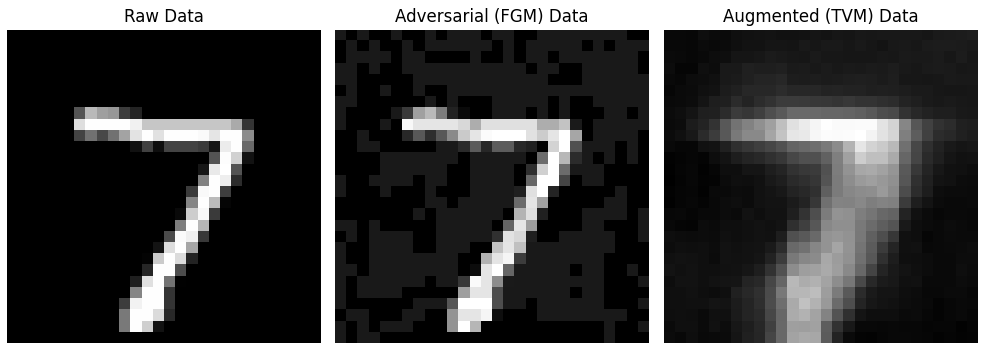
\includegraphics[width=0.6\textwidth]{images/tvm_example.png}
    \caption{}
\end{figure}

\newpage